\documentclass{article}
\usepackage[utf8]{inputenc}
\usepackage[default]{raleway}
\usepackage{pgf-pie,multirow,longtable, tikz, titlesec, comment, tabularx, makecell, float, listings, array, setspace, geometry, graphicx, xcolor, xparse, fancyvrb, relsize, fancyhdr, booktabs, hyperref, eurosym}
%\geometry{a4paper, left=2cm, right=2cm, top=2cm, bottom=2.5cm}
\renewcommand{\headrulewidth}{0pt}

% ----------------------------- Definizione tabella ---------------------------

\newcolumntype{C}[1]{>{\centering\arraybackslash}m{#1}}

% ------------------------------Metadati indice --------------------------------
\title{\textbf{\fontsize{30}{6}\selectfont Indice}}
\author{\fontsize{14}{6}\selectfont ByteOps}
\date{}

% -----------------------------Creazione footer --------------------------------
\pagestyle{fancy} 
\fancyhf{}
\renewcommand{\footrulewidth}{0.4pt} 
\lfoot{ 
    \parbox[c]{2cm}{
\includegraphics[width=2cm]{../Images/logo.png}}
    \textcolor[RGB]{120, 120, 120}{$\cdot$ Piano di progetto}
}
\rfoot{\thepage}

% --------------------------Modifica formato hyperlinks ------------------------
\hypersetup{
    colorlinks=true,
    linkcolor=black,
    filecolor=black,      
    pdftitle={Piano di progetto},
    pdfpagemode=FullScreen,
}

\definecolor{responsabile}{RGB}{0,102,204}
\definecolor{amministratore}{RGB}{0,204,102}
\definecolor{analista}{RGB}{255,165,0}
\definecolor{progettista}{RGB}{255,0,0}
\definecolor{programmatore}{RGB}{128,0,128}
\definecolor{verificatore}{RGB}{255,192,203}



\begin{document}
\pagestyle{fancy}
\begin{center}

\includegraphics[width = 0.7\textwidth]{../Images/logo.png} \\
\vspace{0.2cm}
\textcolor[RGB]{60, 60, 60}{\textit{ByteOps.swe@gmail.com}} \\
\vspace{1cm}
\fontsize{16}{6}\selectfont Piano di progetto \\
\vspace{0.5cm}
\end{center}

\section*{Informazioni documento}
\def\arraystretch{1.2}
\begin{tabular}{>{\raggedleft\arraybackslash}p{0.2\textwidth}|>{\raggedright\arraybackslash}p{0.6\textwidth}c}
\hline
\addlinespace
    \textbf{Redattori} & A. Barutta \\ & R. Smanio \\ & N. Preto \vspace{10pt} \\
    \textbf{Verificatori} & E. Hysa \\ & L. Skenderi \\ & D. Diotto \vspace{10pt} \\
    \textbf{Amministratore} & F. Pozza \vspace{10pt} \\
    \textbf{Destinatari} & T. Vardanega \\ & R. Cardin \vspace{10pt} \\
    \textbf{Partecipanti} & A. Barutta \\ & E. Hysa \\ & R. Smanio \\ & D. Diotto \\ & F. Pozza \\ & L. Skenderi \\ & N. Preto \vspace{10pt} \\
\end{tabular}
\pagebreak 

% ------------------------- Changelog ----------------------------

\begin{tabular}{|C{2.5cm}|C{2.5cm}|C{2.5cm}|C{2.5cm}|C{2.5cm}|}
    \hline
    \textbf{Versione} & \textbf{Data} & \textbf{Autore} & \textbf{Verificatore} & \textbf{Dettaglio} \\
    \hline
    \label{Git_Action_Version} 0.0.2 & 05/11/2023 & Nome autore & Nome verificatore & Aggiunto rischio sezione 2 \\
    \hline 
    0.0.1 & 03/11/2023 & Nome autore & Nome verificatore & Scrittura delle sezioni 1 e 2 \\
    \hline 
 
    
\end{tabular}

\pagebreak

% ------------------------- Generazione automatica indice ----------------------
\setstretch{1.5}
\maketitle
\thispagestyle{fancy}
\tableofcontents
\setstretch{1.2}
\pagebreak

% ---------------------------- Inizio documento -------------------------------

\section{Introduzione}
\subsection{Scopo del documento}
Il presente documento ha lo scopo di identificare la metodologia di pianificazione e illustrare le modalità con cui il gruppo \textit{ByteOps} sta sviluppando il progetto assegnato, al fine di garantire efficacia ed efficienza nel processo di sviluppo.\\
I contenuti che vengono trattati sono:
\begin{itemize}
    \item Analisi dei rischi
    \item Assegnazione ruoli dei membri del gruppo
    \item Descrizione del modello adottato con relative motivazioni della scelta
\end{itemize}


\subsection{Scopo del capitolato}
Il Capitolato C6 affidato al gruppo, si prefigge come obiettivo la realizzazione di una piattaforma di monitoraggio di una \textit{"Smart City"} che consenta di avere sotto controllo lo stato di salute della città in modo tale da prendere decisioni veloci, efficaci ed analizzare poi gli effetti conseguenti.
A tale scopo il proponente richiede di simulare dei sensori posti in diverse aree per reperire informazioni relative alle condizioni della città. 
I dati trasmessi in tempo reale dai sensori devono poter essere memorizzati in modo tale da renderli disponibili per la visualizzazione tramite una dashboard, composta anche da widget e grafici, per una visione d'insieme delle condizioni della città in tempo reale. 
L'applicativo potrà consentire alle autorità locali di prendere decisioni informate e tempestive sulla gestione delle risorse e sull'implementazione di servizi e, inoltre, si potrebbe rivelare uno strumento essenziale per coinvolgere i cittadini nella gestione e nel miglioramento della città.

\subsection{Riferimenti}
\subsubsection{Riferimenti normativi}
\begin{itemize}
\item Norme di progetto
\item \href {https://www.math.unipd.it/~tullio/IS-1/2023/Progetto/C6.pdf} {Capitolato d'appalto C6 - InnovaCity}
\item \href {https://www.math.unipd.it/~tullio/IS-1/2023/Dispense/PD2.pdf} {Regolamento del progetto didattico}
\end{itemize}

%--Il seguente documento è stato redatto con l'obiettivo di valutare e disaminare i potenziali rischi che il gruppo potrebbe affrontare nel corso delle attività di sviluppo del capitolato. In questo documento veranno esposti i vari rischi identificati, accompagnati da una relativa previsione di impatto che ciascuno di essi potrebbe avere e una possibile soluzione.
\section{Calendario di massima del progetto}
\subsection{Introduzione}
Il calendario di massima del progetto illustra le date previste per le revisioni del progetto
alla luce di quanto analizzato nelle sezioni:
\begin{itemize}
    \item Analisi dei rischi;
    \item Analisi dei requisiti;
    \item Pianificazione.
\end{itemize}
\subsection{Prima stesura 25/10/2023}
Il gruppo si pone come obiettivo temporale delle revisioni il seguente calendario:
\begin{table}[ht]
    \centering
    \begin{tabular}{|c|c|}
        \hline
        \textbf{Revisione} & \textbf{Data} \\
        \hline
        Requirements and Technology Baseline & 20/12/2023 \\
        Product Baseline  & 29/03/2024 \\
        Customer Acceptance & 30/05/2024 \\
        % Aggiungi altre revisioni e date secondo necessità
        \hline
    \end{tabular}
    \caption{Calendario delle Revisioni}
\end{table}
\section{Stima dei costi di realizzazione}
\subsection{Introduzione}
La stima dei costi di realizzazione è la stima del budget totale necessario per la realizzazione del progetto alla luce di quanto analizzato in :
\begin{itemize}
    \item Analisi dei rischi;
    \item Analisi dei requisiti;
    \item Preventivo costi e assunzioni impegni.
\end{itemize}

\subsection{Prima Stesura 25/10/2023}
\begin{center}
        
    \begin{tabular}{|C{3cm}|C{2cm}|C{2cm}|C{2cm}|C{2cm}|C{2cm}|}
        \hline

        \textbf{Ruoli} & \textbf{Costo orario} \linebreak \textit{(\euro\ / h)} & \textbf{Ore previste per ruolo} & \textbf{Ore previste per membro} & \textbf{Costo per ruolo} \linebreak \textit{(\euro\ )} \\
        \hline\hline
        
        Responsabile & 30 & 49 & 7 & 1470 \\
        \hline
        
        Amministratore & 20 & 49 & 7 & 980 \\
        \hline
        
        Analista & 25 & 63 & 9 & 1575 \\
        \hline 
        
        Progettista & 25 & 210 & 30 & 5250 \\ 
        \hline
        
        Programmatore & 15 & 105 & 15 & 1575 \\
        \hline
        
        Verificatore & 15 & 175 & 25 & 2625 \\
        \hline\hline
        
        \textbf{TOTALE} & - & 651 & 93 & 13475 \\
        \hline
    \end{tabular}
    \end{center}

    \begin{figure}[h]
        \centering
        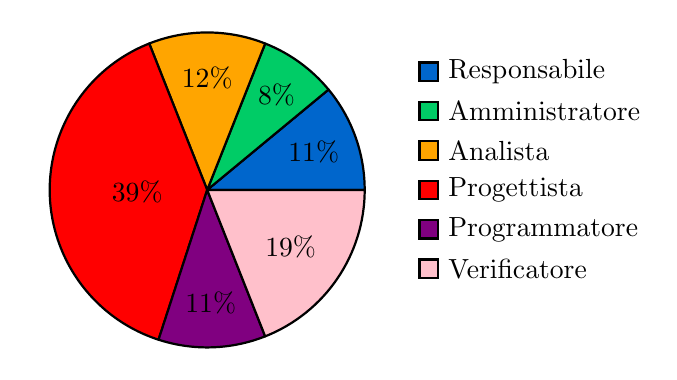
\begin{tikzpicture}
            \pie[
                text=legend,
                color={responsabile, amministratore, analista, progettista, programmatore, verificatore},
                radius=2, % Imposta il raggio per rendere il grafico circolare
                line width=0pt % Rimuovi i contorni
            ]{11/Responsabile, 8/Amministratore, 12/Analista, 39/Progettista, 11/Programmatore, 19/Verificatore}
        \end{tikzpicture}
        \caption{Distribuzione dei costi per ruolo}
    \end{figure}
    
    Il totale identificato di 13475\euro\ verrà considerato come limite di budget invalicabile,
    nel caso ci fosse il rischio di superamento del budget verranno negoziati al ribasso i requisiti
    di progetto.
\subsection{Seconda Stesura 16/12/2023}
Dopo una dettagliata rivalutazione dei requisiti e un'analisi con il committente, la stima dei costi è stata riesaminata. Ciò ha comportato la modifica delle ore dedicate alla progettazione e alla programmazione, portando così al nuovo costo di 12565\euro\ .
\begin{center}
        
    \begin{tabular}{|C{3cm}|C{2cm}|C{2cm}|C{2cm}|C{2cm}|C{2cm}|}
        \hline

        \textbf{Ruoli} & \textbf{Costo orario} \linebreak \textit{(\euro\ / h)} & \textbf{Ore previste per ruolo} & \textbf{Ore previste per membro} & \textbf{Costo per ruolo} \linebreak \textit{(\euro\ )} \\
        \hline\hline
        
        Responsabile & 30 & 49 & 7 & 1470 \\
        \hline
        
        Amministratore & 20 & 49 & 7 & 980 \\
        \hline
        
        Analista & 25 & 63 & 9 & 1575 \\
        \hline 
        
        Progettista & 25 & 140 & 20 & 3500 \\ 
        \hline
        
        Programmatore & 15 & 161 & 23 & 2415 \\
        \hline
        
        Verificatore & 15 & 175 & 25 & 2625 \\
        \hline\hline
        
        \textbf{TOTALE} & - & 651 & 93 & 12565 \\
        \hline
    \end{tabular}
    \end{center}

    \begin{figure}[h]
        \centering
        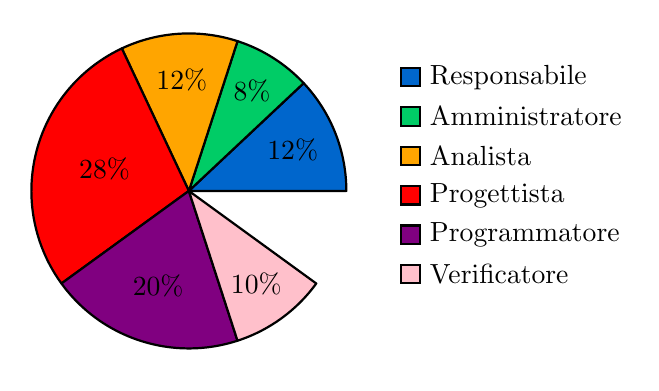
\begin{tikzpicture}
            \pie[
                text=legend,
                color={responsabile, amministratore, analista, progettista, programmatore, verificatore},
                radius=2, % Imposta il raggio per rendere il grafico circolare
                line width=0pt % Rimuovi i contorni
            ]{12/Responsabile, 8/Amministratore, 12/Analista, 28/Progettista, 20/Programmatore, 10/Verificatore}
        \end{tikzpicture}
        \caption{Distribuzione dei costi per ruolo aggiornameto 16/12/2023}
    \end{figure}

\section{Analisi dei rischi}
\subsection{Rallentamento delle attività}
Uno dei principali rischi che potrebbero manifestarsi è l'armonizzazione tra le attività personali con quelle attività progettuali. Tale rischio
potrebbe causare un rallentamento nell'esecuzione dei compiti assegnati ai membri del gruppo, con conseguente rallentamento del processo di sviluppo. 
Si prevede che questo rischio si intensificherà durante il periodo di sessione invernale 2023-2024, a causa degli impegni legati agli esami.\\ 
Per quanto riguarda le possibili soluzioni per attenuare il problema, si propone: 

\begin{itemize}
    \item Una buona organizzazione tra i membri del gruppo per garantire una distribuzione equa del lavoro da svolgere.
    \item La creazione di un ambiente di lavoro asincrono, in modo da permettere lo svolgimento dei compiti assegnati da parte di ciascun membro del gruppo secondo le proprie tempistiche.
\end{itemize}

\subsection{Apprendimento ed utilizzo delle nuove tecnologie}
L’apprendimento e l'implementazione delle tecnologie proposte possono rappresentare un rischio considerevole per lo 
sviluppo di un progetto, in quanto esista la possibilità che lo studio accurato di queste tecnologie richieda più tempo del previsto. \\
Per quanto riguarda le possibili soluzioni per attenuare il problema, si propone:
\begin{itemize}
    \item Pianificazione accurata del tempo necessario per l’assimilazione e l’implementazione \\delle nuove tecnologie.
    \item Sfruttare le competenze individuali di ciascun membro del gruppo, al fine di accelerare \\ il processo di apprendimento.
    \item Approfittare, ove possibile, delle opportunità di formazione offerte dall’azienda proponente, in modo da risolvere eventuali dubbi e consolidare i concetti appresi.
\end{itemize}
\subsection{Inefficacia della comunicazione} 
L’inefficacia della comunicazione tra i componenti del gruppo potrebbe condurre a ritardi significativi nello sviluppo del progetto. Questo rischio assume una rilevanza particolare considerando la natura collaborativa del lavoro di gruppo, che richiede l’adesione a norme concordate collettivamente.
\\Per quanto riguarda le possibili soluzioni per attenuare il problema, si propone:
   \begin{itemize} 
    \item Impiego di strumenti di comunicazione efficaci e l’istituzione di regole chiare per le riunioni e le discussioni tra i componenti del gruppo.
    \item Incentivare un ambiente di lavoro che favorisca la collaborazione e sia aperto all'espres-sione di idee o feedback da parte dei membri del gruppo.
\end{itemize}


\section{Pianificazione}
\subsection{Introduzione}
In conformità con la filosofia di sviluppo moderna e dinamica, abbiamo scelto di adottare il modello agile, con un focus specifico sul framework Scrum.
Lo Scrum, con le sue pratiche iterative e collaborative, offre una risposta efficace alle sfide e alle mutevoli esigenze del mondo contemporaneo dello sviluppo software.\\
Attraverso l'implementazione di Scrum, il nostro team mira a ottenere numerosi benefici positivi che influenzeranno in modo significativo il successo del progetto.
\\
\\
\textbf{Vantaggi del Modello Agile e Scrum}
\\L'adozione del modello Agile, e in particolare di Scrum, introduce una serie di lati positivi che contribuiranno al raggiungimento dei nostri obiettivi di progetto.
Alcuni dei principali vantaggi che ci aspettiamo di acquisire includono:

\begin{itemize}
    \item \textbf{Flessibilità e Adattabilità:} Lo Scrum consente una rapida risposta ai cambiamenti nei requisiti del cliente, garantendo una maggiore flessibilità durante tutto il ciclo di sviluppo;
    \item \textbf{Collaborazione e Comunicazione:} La struttura collaborativa di Scrum promuove una comunicazione aperta e continua tra i membri del team e le parti interessate, migliorando la comprensione reciproca e la condivisione di conoscenze;
    \begin{itemize}
        \item In particolare con l'azienda proponente sono fissati SAL (Stato avanzamento lavori) ogni due settimane.
    \end{itemize}
    \item \textbf{Consegna Incrementale:} Attraverso la pratica di rilasci incrementali, Scrum consente la distribuzione graduale delle funzionalità, fornendo valore al cliente fin dalle prime fasi del progetto;
    \item \textbf{Miglioramento Continuo:} Le retrospettive regolari incoraggiano il miglioramento continuo del processo, permettendo al team di identificare e risolvere eventuali problematiche in modo tempestivo.
\end{itemize}

La scelta di adottare il modello Agile con Scrum riflette la nostra dedizione a fornire un prodotto di qualità, rispondendo in modo efficiente ai cambiamenti e alle esigenze del cliente.


\subsection{Requirements and Technology Baseline}
\subsubsection{Primo periodo  06/11/2023 - 24/11/2023}
\begin{longtable}{|C{3cm}|C{3cm}|C{1cm}|C{1.5cm}|C{2cm}|C{1.5cm}|C{2cm}|}
    \hline

    \textbf{Ambito} \linebreak \textbf{(Ruolo)}  & \textbf{Avanzamento atteso}  & \textbf{Fatto} & \textbf{Ore previste} \linebreak \textit{Task + verifica} & \textbf{Costo} \linebreak \textit{((Task + verifica) \euro\ )} & \textbf{Ore effettive} \textit{Task + verifica} & \textbf{Costo effettivo} \linebreak \textit{((Task + verifica) \euro\ )} \\
    \hline\hline
    
    \multirow{6}{*}{Norme di progetto} & Sez. Introduzione & Si & 2+1 & - & 2+1 & - \\
    \cline{2-7}
    
    & Sez. Documentazione & Si & 3+1 & - & 3+1 & - \\
    \cline{2-7}
    
    & Sez. Sviluppo & Si & 3+1 & - & 3+1 & - \\
    \cline{2-7} 
    
    & Sez. Gestione della configurazione & Si & 2+1 & - & 2+1 & - \\
    \cline{2-7}
    
    & Sez. Processi organizzativi & Si & 3+1 & - & 3+1 & - \\
    \cline{2-7}
    
    & Sez. Verifica (Documentazione)  & Si & 1+1 & - & 1+1 & - \\
    \hline
    \multirow{1}{*}{Altro} & Creazione template LaTeX per i verbali & Si & 1+1 & - & 1+1 & - \\
    \hline  

    \multirow{3}{*}{\parbox{3cm}{Analisi dei requisiti \\ (Analisti)}} & Sez. Use case & Si & 6+2 & 150+30 & 7+2 & 175+30 \\
    \cline{2-7}
    
    & Sez. User story & Si & 4+1 & 100+15 & 5+1 & 125+15 \\
    \cline{2-7}
    
    & Sez. Requisiti funzionali & Si & 4+1 & 100+15 & 4+1 & 125+15 \\
    \hline  
    
    \multirow{5}{*}{\parbox{3cm}{Piano di progetto \\ (Responsabile)}} & Sez. Introduzione & Si & 1+1 & 30+15 & 1+1 & 30+15 \\
    \cline{2-7}
    
    & Sez. Calendario di massima del progetto & Si & 1+1 & 30+15 & 1+1 & 30+15 \\
    \cline{2-7}
    
    & Sez. Stima dei costi di realizzazione & Si & 1+1 & 30+15 & 1+1 & 30+15 \\
    \cline{2-7}
    
    & Sez. Analisi dei rischi & Si & 2+1 & 60+15 & 2+1 & 60+15 \\
    \cline{2-7}
    
    & Sez. Pianificazione: (Primo periodo) & Si & 2+1 & 60+15 & 2+1 & 60+15 \\
    \hline  
    
    \multirow{2}{*}{\parbox{3cm}{POC \\ (Programmatori)}} & Simulazione di almeno un sensore in Python & Si & 2+1 & 30+15 & 2+1 & 30+15 \\
    \cline{2-7}
    
    & Connessione containerizzata Docker  (Python, Kafka, ClickHouse (Opzionale)) & Si & 3+1 & 45+15 & 4+1 & 60+15 \\
    \hline  
    
    \multirow{2}{*}{\parbox{3cm}{ Amministrazione \\ (Amministratori)}} & Automatizzazione compilazione file LaTeX & Si & 5+1 & 100+15 & 7+1 & 140+15 \\
    \cline{2-5}
    
    & Automatizzazione rinomina file sulla base della versione & Si & 3+1 & 60+15 & 4+1 & 80+15 \\
    \hline 
    
   
    
    \textbf{TOTALE} & - & - & - & 990 & - & 1140\\
    \hline
\end{longtable}

\subsubsection*{Rischi occorsi, impatto, mitigazione}

Nel corso del primo periodo, si sono presentate le seguenti problematiche:
\begin{itemize}
    \item \textbf{Inesperienza nell'uso dell'ambiente Docker}
    \begin{itemize}
        \item \textbf{Impatto:} Rallentamento delle attività di sviluppo del Proof of Concept (PoC);
        \item \textbf{Mitigazione:}  È stata avanzata una richiesta al proponente per la realizzazione di un corso di formazione su Docker.
    \end{itemize}
    \item \textbf{Dubbi relazioni tra casi d'uso:}
    \begin{itemize}
        \item \textbf{Impatto:} Sebbene la definizione dei casi d'uso sia stata completata, la correttezza è risultata dubbia;
        \item \textbf{Mitigazione:} È stata richiesto un incontro con il Prof. Cardin per chiarimenti e approfondimenti.
\end{itemize}
\end{itemize}



\end{document} 